\documentclass[11pt,a4,epsf]{report}
%\documentstyle[11pt]{j-article}
%\usepackage{otf}
\usepackage{amssymb}
\usepackage{theorem}
\usepackage{ascmac} %itembox
\usepackage[titletoc,title]{appendix}
\usepackage[dvipdfmx]{graphicx}
%%% for apple LaserWriter Series %%
%% 
\setlength{\topmargin}{-0.5in}
\setlength{\textwidth}{5.6in}
\setlength{\textheight}{8.8in}
\setlength{\oddsidemargin}{0.35in}
\setlength{\evensidemargin}{0in}

\setlength{\topmargin}{-1cm}
\setlength{\oddsidemargin}{0cm}
\setlength{\textwidth}{16cm}
\setlength{\textheight}{24cm}
\renewcommand{\@}[1]{{\bf #1}}

\title{{\bf IoT デバイス・プログラミング}}
\author{下薗 真一\\
e-mail: {\sf sin@ai.kyutech.ac.jp}\\
}
%\date{}
%
% 諸定義
%
\def\linesparpage#1{\baselineskip=\textheight\divide\baselineskip#1}
\newtheorem{exerc}{演習}
\newtheorem{adv}{発展課題}

%%%%%%%%%%%%%%%%%%%%%%%%%%%%%%%%%%%%%%%%%%%%%%%%%%%%%%%%%%%%%%%%%%%%%%
%%%%% ワンポイントの表示 %%%%%%%%%%%%%%%%%%%%%%%%%%%%%%%%%%%%%%%%%%%%%
\newcounter{pntnumber}
\setcounter{pntnumber}{0}
\newcommand{\POINT}[2]{
 \medskip
 \refstepcounter{pntnumber}
\noindent
■■■■■ {\sf Point \arabic{pntnumber}:} {\bf #1} \hrulefill ■ \\
{\small #2}

\noindent
■ \hrulefill ■■■■■ \\
% \begin{center}
%  \fbox{
%   \begin{minipage}{\textwidth}
%    \noindent
%    {\bf ポイント \arabic{pntnumber} (#1)}
%    #2
%   \end{minipage}
%  }
% \end{center}
 \medskip
}
%%%%%%%%%%%%%%%%%%%%%%%%%%%%%%%%%%%%%%%%%%%%%%%%%%%%%%%%%%%%%%%%%%%%%%
%
% 本文
%
\begin{document}
%\linesparpage{40}
\linesparpage{36}
\maketitle

\medskip

\begin{description}
\item[対象:] 知能情報工学科 2 年次
\item[期間:] 前期
\item[機材:] ???CAD実験室(共通教育研究棟 3 階 S303 室)の Linux PC 端末%\\
%	初回のみ 第 I 計算機室(研究棟 6 階)の Linux PC 端末
\end{description}

\medskip

\section{演習の目標}

ワンボード PC である Raspberry Pi をエッジ(末端)デバイスとし,
エッジデバイス上の各種センサーを使った測定,表示出力の使用,
インターネット上のサービスとの連携,などについてプログラミング演習を行う.
IoT とよばれる概念とそこで必要となる技術を習得する.

センサーボードのライブラリによる使用に必要なスクリプト言語 Python にふれる.
プログラミング言語によらない,プログラミングやコンピュータサイエンスの概念を再認識する.

\section{IoT とは}

IoT とは,Internet of the Things (もののインターネット)の略である.
インターネットを,ユーザー(人)が他のユーザーあるいはその集合と情報をやりとりするための空間としてだけではなく,
デバイスや装置が他のデバイス・装置あるいはユーザーとインターネットを通じて情報をやりとりする空間として考えること,
またこれにより実現できるようになる技術やサービスのことを指す.

従来は,デバイスや装置などは,電話回線,無線通信,有線回線などで専用の回線やネットワークを構築し,通信を行うのが主であった.
しかし,有線および無線でのインターネット・インフラが整備され,
機器の基本ソフトウェアとして TCP/IP を使える OS が一般的になり,
公開鍵暗号などセキュアな通信経路を確保するための CPU パワーが安価になったことなどから,
機器間,あるいは機器とユーザーの間の接続をインターネットで行い,一般的な回線で多様な機器間で情報をやりとりし,
よりすすんだサービスを提供したり,技術を可能にしようという考え方がひろまってきた.
5G などのより高速で低遅延の無線インターネット回線が実現すれば,ますます発展すると考えられている.

ただし,現在すでに直接ユーザーが使用し状況を確認するわけではない膨大な量の機器や装置が初期設定のままインターネットに接続される状況になっており,
セキュリティ上の脆弱性を悪用され,社会インフラへの攻撃などが起きるのではないか,という懸念が残っている.

\section{Raspberry Pi}

Raspberry Pi ラズベリー・パイは,子供の教育目的にイギリスで設計され世界的に普及しているワンボードPCである.
Linux などを動作させることができる CPU (ARM7相当)とメモリをそなえ, 基本ディスク装置として SD カードを使用する.
ビデオ出力(HDMI / アナログビデオ),音声出力,キーボードやマウスを接続できる USB ポート,有線/無線のイーサネットインターフェースを備え,micro USB ポートから電源を供給し,ディスプレイ,キーボードやマウスを接続すれば,
LINUX や組み込み Windows が動作する単体のパソコンとして使用することができる.
また,汎用の I/O ポートやIC間通信のバスが物理的に利用者に開放されており,自作の電子回路や市販のセンサーボードなどハードウェアを追加し使用することができる.

今回は,Sensor Hat  とよばれる,センサ類とスイッチを入力として持ち,マトリクス LED を出力として備える市販のボードを Raspberry Pi にとりつけて演習を行う.


\section{Python 言語}

本演習では,Python 3.x を使用する.

Linux などマルチタスク,マルチユーザーをサポートする OS では,一般に仮想メモリが実装される.
メモリー空間に配置された入出力アドレスへのアクセスには,仮想メモリの影響の排除や他のプロセスのアクセスとの調停が必要になるため,ハードウェアとの通信は,OS の利用を前提としないワンチップ・マイコンより複雑にならざるをえない.
たとえ 1 ビットの読み書きでも,ライブラリを使うことが前提となる.
この実験で使用する Sensor Hat には,使いやすいライブラリが Python 言語で提供されており,入出力やセンサーとの通信プロトコルについては気にせず利用できるようになっている.
そこで,この演習のプログラミングは Python 言語で行う.

Python 言語は,インタープリタで動作する,インデンテーション言語である.
予約語や式,演算子は C言語などに近い.
豊富なライブラリやツールが公開され,それらの追加インストールが容易で,スクリプトの記述から,インターネットでのデータスクレイピング,深層学習によるデータ処理まで,さまざまなデータ処理に使われている.

すでに C 言語を学んでいる場合,Python プログラミングを基礎から体系的に学ぶのはやや冗長である.
今回は Sensor Hat の基本的な使い方を学ぶ中で, C 言語ほか既知のプログラミング言語との相違をふまえる形式で修得する.

\subsection{Python と C の違い,初級編}
%\begin{table}[h]
  \begin{tabular}{|p{1.5in}|p{2in}|p{2in}|}
\hline
文法,記述法 & Python 言語 & C/C++ 言語 \\
\hline
\hline
文の終わり,区切り & 改行 (式の途中でない限りテキスト中の1行が1文) & \verb+;+(セミコロン) \\
\hline
実行ブロック & 連続して行頭からのインデント文字数が同じ文 & 一文,または \verb+{+ から \verb+}+ の間\\
\hline
コメント & \verb+#+ の後文末まで & \verb+/*+ から \verb+*/+ の間,\par \verb+//+ の後文末まで \\
\hline
演算子 & インクリメント,デクリメントはない &  \\
\hline
条件分岐 & \verb+if 条件式 :+\par ~~~ブロック \par\verb+else:+ \par ~~~ブロック & \verb+if (条件式) +\par ブロック\par\verb+else+\par ブロック \\
\hline
明示的な制御変数を持つループ & \verb+for 変数/変数の組 in データのコレクション :+ \par ~~~ブロック& \verb+for (初期化式,条件式,更新式)+ \par ブロック \\
\hline
ループを一度実行した後に条件判断をするループ & なし & \verb+do ... while+ 文\\
\hline
組み込みのデータのコレクションの型 & 組(固定長,変更不可),配列,リスト,辞書,集合,整数範囲 & 配列,構造体(クラス)\\
\hline
データのコレクションの大きさ,要素数 & \verb+len(コレクション)+ & 配列の長さはメモリ割り当て時以外不明,プログラマが管理\\
\hline
  \end{tabular}
%\end{table}

\section{Raspberry Pi の基本,起動からシャットダウン(電源投了)まで}

Raspberry Pi の HDMI ポートと USB ポート,ネットワークポートを使えば,ディスプレイ,キーボード,マウスを接続しインターネットに接続した PC として使用できるが,今回はトラブル等が発生しない限り,ディスプレイおよびキーボードのない状態で起動し,
Wi-Fi を通じて端末エミュレーターで接続し,その中ですべての作業を行う.

\subsection{電源投入,起動と端末エミュレータからのログイン}

Raspberry Pi には電源スイッチはない.
電源入力である micro USB ポートに,5V/2A の USB電源からケーブルをつないだ時点で起動する.
HDMI やシリアル入出力を通してディスプレイ装置を接続している場合,Linux の起動プロセスメッセージが表示される.
この実験で使用する micro SD カードには, (1)  Wi-Fi 接続を行い,(2) X ウインドウを使用しない状態でログインを待機し,また (3) ネットワークからの SSH 接続を受け入れる設定で Linux (Debian ベースの Raspbian) が起動するようになっている.
SenseHat を装着した状態では,LED マトリクスが消灯したころが起動プロセスが終了したころである.

接続先の Raspberry Pi の IP アドレスが \verb+192.168.1.129+ であるとする.
(実際に使用する IP アドレスは,micro SD カードで OS から設定されるか,ネットワークのアドレスサーバ(DHCP)から割り当てられるので,各自確認すること.)
端末エミュレータからの接続は,セキュアシェル ssh コマンドを使って次のように行う.
\begin{quote}
\small
\begin{verbatim}
$ ssh 192.168.1.129 -l pi
pi@192.168.1.129's password: 

Linux raspberrypi 4.14.98-v7+ #1200 SMP Tue Feb 12 20:27:48 GMT 2019 armv7l
(省略)
pi@raspberrypi:~ $ 
\end{verbatim}
\end{quote}
\verb+pi+ は OS インストール時にデフォルトで設定されるユーザー名で,パスワードは \verb+raspberry+ である.
bash のコマンドプロンプト \verb+pi@raspberrypi:~ $+ で,raspberrypi という名前のホストに ユーザー名 pi でログインしている状態であることがわかる.
\verb+pi+ は管理グループユーザーに設定されているため,管理権限が必要なコマンドも \verb+sudo [コマンド]+ で使用することができる.

\subsection{Python 3 のインタラクティブモードの実行と終了}

Python は,シェルと同様にプログラム・ファイルを実行することができ,インタラクティブ・モードで使うこともできる.
Python 3.x のインタラクティブモードでの起動,対話的実行,終了は,以下のように行う.
実行は,文(改行するまで)ごとに行われる.
\begin{quote}
\small
\begin{verbatim}
pi@raspberrypi:~ $ python3
Python 3.5.3 (default, Sep 27 2018, 17:25:39) 
[GCC 6.3.0 20170516] on linux
Type "help", "copyright", "credits" or "license" for more information.
>>> print("Hello, world!")
Hello, world!
>>> pi = 4
>>> sgn = -1
>>> for i in range(1,1000):
...    prev = pi                       # ← ... の後に空白 3 つ
...    pi = pi + 4.0*sgn/(2*i+1)       # 上に同じ
...    sgn = -sgn
...                                   # ← ... の後になにも入力せず改行
>>> print((prev+pi)/2)
3.141593154089919
>>> 
>>> quit()
pi@raspberrypi:~ $ 
\end{verbatim}
\end{quote}
\verb+>>>+ はインタプリタのプロンプトである.
\verb+...+ は,改行したがまだループのネストの中にあり,最も外側の文が終わっていないことを示しているので,ネストのレベルにあわせた適切な量の空白やタブを入れインデントづけする.
上の例では,\verb+for in range(1,1000) :+ で変数 \verb+i+ に範囲 $[1,1000)$ から順に一つずつ整数を代入し,
その次の同じインデントを持つ 4行をくりかえす.
インタラクティブモードでは,ループの中のブロックが終了したことを伝えるため,\verb+...+ のあとをカラのまま改行して, \verb+for+ の文を終わらせる.

Python のインタラクティブモードを終了するには,関数 \verb+quit()+ を実行する.

\begin{excercise}
Python 3 のインタプリタモードで上記のプログラムを実行し,ループの \verb+i+ の範囲を 1 から 9999 までにして \verb+pi+ の値がどのように変化するか確かめなさい.
その後,Python を正しく終了させなさい.
また,ctrl-C で終了できるかどうか確かめなさい.
\end{excercise}

\subsection{シャットダウンと終了}

Raspberry Pi の電源を切る場合,OS のシャットダウンを使用してから micro USB ケーブルを抜く.
\begin{quote}
\small
\begin{verbatim}
pi@raspberrypi:~ $ sudo shutdown now
Connection to 192.168.1.129 closed by remote host.
Connection to 1192.168.1.129 closed.
$ 
\end{verbatim}
\end{quote}
ディスプレイがないと OS のシャットダウンメッセージを見ることはできないが,
上記方法で接続を切ってからしばらくすると LED の点滅をしなくなるので,ケーブルを抜いて終了する.

ただしディスクアクセス中などでなければ,突然電源を OFF にしてもファイルやディレクトリが壊れたり,起動しなくなる,といった状態になることはまれである.


\section{Sensor Hat の使い方}

\subsection{LED マトリクスによるテキストの流れ表示}

Python のインタラクティブモードで,Sensor Hat の LED マトリクス表示装置を使用してみよう.
\begin{quote}
\small
\begin{verbatim}
pi@raspberrypi:~ $ python3
Python 3.5.3 (default, Sep 27 2018, 17:25:39) 
[GCC 6.3.0 20170516] on linux
Type "help", "copyright", "credits" or "license" for more information.
>>> from sense_hat import SenseHat        # SenseHat クラスライブラリの使用を宣言
>>> sense = SenseHat()                    # SenseHat へのアクセスオブジェクトを生成
>>> sense.show_message("hello, world!")   # LED Matrix に文字列を流れ出力
>>> 
\end{verbatim}
\end{quote}

\begin{excercise}
流れるスピード,文字の色,背景の色,上下の方向などが設定/変更できるので,\verb+show_message+ 関数の引数を Web ページ\footnote{Google 等で検索しなさい.たとえば {\tt https://pythonhosted.org/sense-hat/api/} など}でしらべ,メッセージや色を変えてみなさい.
\end{excercise}

\subsection{慣性計測センサ(IMU)}

SenseHat には,マイクロマシン技術を使った超小型の一体型加速度,ジャイロ(回転),磁気のセンサが搭載されている.
このようなセンサの普及によって,カメラの手ぶれ防止やドローンの自動制御,スマートホンの万歩計機能や地図の方位機能が使用可能になった.

下記のコードを実行すると、ctrl-C で中断するまで加速度センサの値を出力しつづける.
\begin{quote}
\small
\begin{verbatim}
>>> from sense_hat import SenseHat 
>>> import time
>>> sense = SenseHat() 
>>> while True :
...    accl = sense.get_accelerometer_raw()
...    msg = "x: {0}, y: {1}, z: {2}".format(accl["x"],accl["y"],accl["z"])
...    print(msg)
...    time.sleep(0.5)
...
0.0058187018148601055 -0.1268848180770874 1.0050058364868164
0.013334525749087334 -0.13098566234111786 0.9833167791366577
0.014061863534152508 -0.13122688233852386 0.9806361198425293
(以下略)
\end{verbatim}
\end{quote}
\verb+変数[キー値]+ は,辞書データ構造のもつ特定のキー値に対応する値を返す.
\verb+文字列.format(値0, 値1, ...)+ は文字列の \verb+{添え字}+ の箇所に、引数にとる値を順に添え字 0 から対応させ埋め込んだ文字列を返す.
辞書は,リスト, 組, 集合などと同様に組み込みのデータ型の一つである.
文字列は \verb+' '+でくくることもできる.

\begin{excercise}
Raspberry Pi の向きを変えて,加速度センサの読み取り値が変化するのを確認し.またそのような値になる理由を考えなさい.
\end{excercise}

\subsection{気温,湿度,気圧センサ}

次に,Python のプログラムをプログラムファイルとして作成しよう.
気候に関する気温,湿度,気圧センサーの値を利用するプログラムを以下に示す.

以下の内容のテキスト・ファイルを Raspberry Pi で作成し,たとえば \verb+sensehat.py+ として(Raspberry Pi のディレクトリに)保存する.
エディタは Raspbian に標準でインストールされている \verb+nano+,または 追加インストールされている \verb+emacs+ を使用するとよい.
\verb+nano+ は使用するコマンド(保存,終了など)がスクリーン下にメニュー形式で表示される.
保存ファイル名を保存時にプロンプトされるので,修正の必要がなければそのまま改行する.
 \begin{itembox}[l]{\tt sensehat.py}
\begin{quote}
\small
\begin{verbatim}
from sense_hat import SenseHat
from datetime import datetime

sense = SenseHat()
sense.clear()

temp = sense.get_temperature()
humi = sense.get_humidity()
pres = sense.get_pressure()
    
print(datetime.now())
print(temp, humi, pres)
\end{verbatim}
\end{quote}
\end{itembox}

Python プログラム・ファイルは,コマンド \verb+python3 [ファイル名] [引数]+ で実行する.
\verb+sensehat.py+ は引数を使わないので,実行例は以下のようになる.
\begin{quote}
\small
\begin{verbatim}
pi@raspberrypi:~/Documents $ python3 sensehat.py 
34.04765701293945  31.003049850463867  1010.461181640625 
pi@raspberrypi:~/Documents $ 
\end{verbatim}
\end{quote}
\verb+from datetime import datetime+ では,ライブラリの \verb+datetime+ モジュールから日時,現在の時間などを扱うための \verb+datetime+ クラス\footnote{データ型とその型用の関数をまとめたものをクラスという. Python や C++ では,データ型やその型の変数の関数を呼び出すとき,コンマでつないで関数を書く.}を導入している.
\verb+.now()+ 関数で現在の日付と時刻を取得できる.あらかじめ決まった表示形式に変換するには,\verb+.strftime+関数を使うとよい.

\subsection{Joystick スイッチ}
SenseHat は, 4方向+押し込みの入力ができるスイッチをもっており,センサと同様に状態を読み取ることができる.
この Joystick スイッチを使えば,キーボードやマウスを接続しなくても, SenseHat だけで直接ユーザーに入力させることができる.

\begin{figure}
\centering
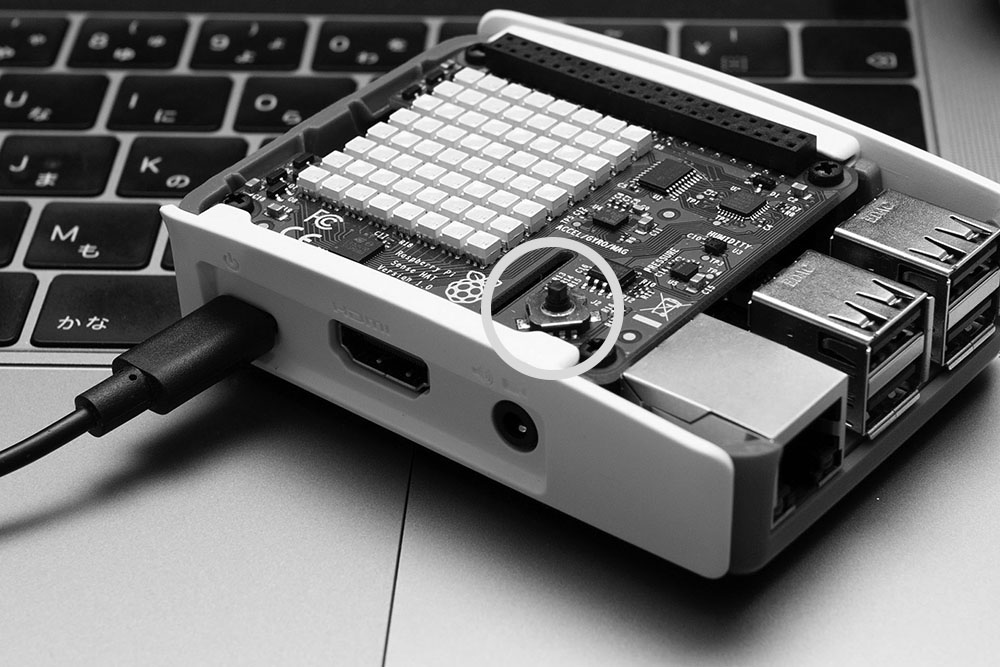
\includegraphics[width=4cm]{joystick.jpg}
%\caption{}
\end{figure}

Joystic スイッチからは,イベントとしてスイッチの変化が起きた時刻,上下左右の4方向または中央のスイッチの種類,押下または解放 の3つ組みを列として得ることができる.
\begin{itembox}[l]{\tt sensehat.py の最後に追加}
\begin{quote}
\small
\begin{verbatim}
while True :
       for event in sense.stick.get_events():
        print(event.timestamp, event.direction, event.action)
    time.sleep(0.5)
\end{verbatim}
\end{quote}
\end{itembox}

\begin{excercise}
Joystick の操作で LED Matrix に流れるメッセージの内容や流れる方向を変更するプログラムを書きなさい.
\end{excercise}


\section{Raspberry Pi とのファイルのやりとり}

Raspberry Pi の SDカード内のディレクトリからファイルを演習端末のディレクトリへコピーする,またその逆を行うには,
端末エミュレータのスクリーン文字をエディタ使用中にコピー/ペーストするほかに,
セキュアシェル \verb+ssh+ の機能を使ったファイル転送を行う \verb+sftp+ コマンドが使用できる.

ファイルの Raspberry Pi へのアップロードまたはダウンロードを行うには,次の手順を踏とよい.
\begin{enumerate}
\item
演習端末の端末エミュレータのシェルで,やりとりするファイルのディレクトリに移動する.
\item
\verb+sftp pi@[アドレス]+ でそのアドレス(の Raspberry Pi)に接続する.
\verb+ls+や\verb+cd+コマンドが使用できるので,カレントディレクトリなどを確認する.
\item
接続直後はログイン直後の状態と同じで,カレントディレクトリはホームディレクトリになっている.
まず,アップロード先あるいはダウンロードするファイルのあるディレクトリに移動する.
アップロードするときは \verb+put [ファイル名]+ コマンドを、ダウンロードするときは \verb+get [ファイル名]+ コマンドを実行する.
ファイル名のファイルがない場合は,エラーになる.
\end{enumerate}
アップロードしているのか,ダウンロードしているのかに注意して作業すること.
間違えると,古いファイルで上書きしてしまうことになる.

\begin{excercise}
演習で作成したファイルを,続きの作業をするため,またレポート作成で参照するために,演習端末のディレクトリにコピーし,
自分の USB メモリにコピーしなさい.
\end{excercise}

\section{センサーデバイス・プログラムの作成}

\end{document}


